% NeurIPS Best Paper Style – clean, flat, minimal
\definecolor{NBlue}{HTML}{1A56A0}
\definecolor{NRed}{HTML}{C0392B}
\definecolor{NGreen}{HTML}{1A7A45}
\definecolor{NGold}{HTML}{B07D1A}
\definecolor{NSlate}{HTML}{4A5568}
\definecolor{NBlueFill}{HTML}{EBF2FB}
\definecolor{NRedFill}{HTML}{FBEAEA}
\definecolor{NGreenFill}{HTML}{EBF5EF}
\definecolor{NGoldFill}{HTML}{FDF6E3}
\definecolor{NSlateFill}{HTML}{F0F2F5}
\definecolor{NStroke}{HTML}{BBBDC2}

\begin{figure}[t!]
\centering
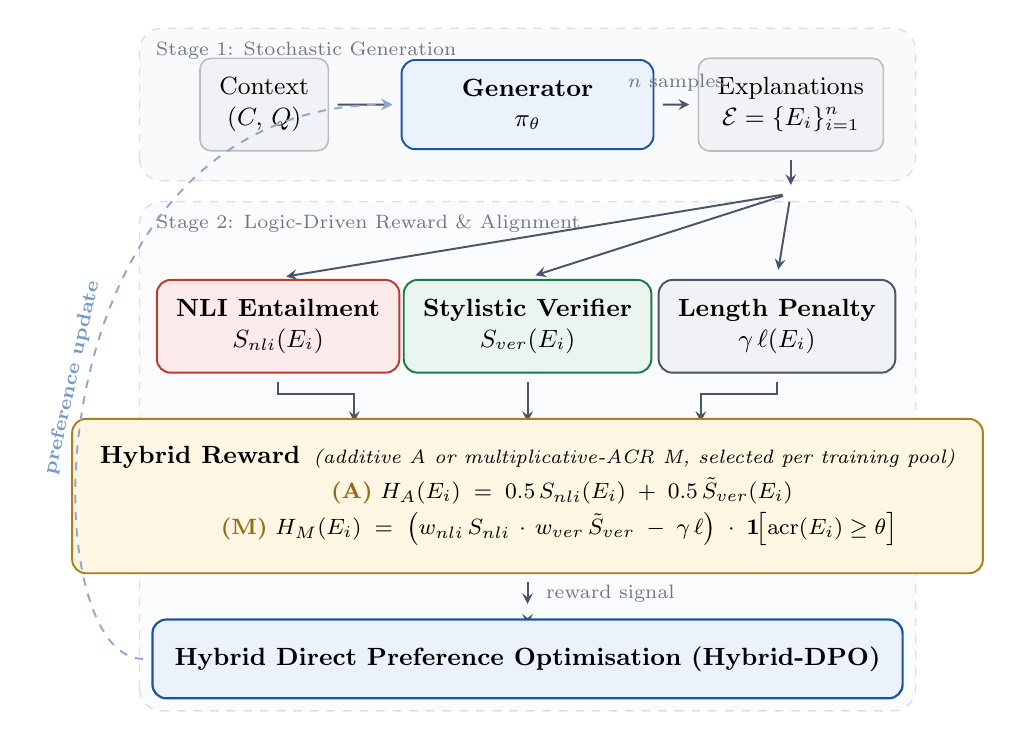
\begin{tikzpicture}[
    scale=0.88,
    >=stealth,
    % Core node styles
    iobox/.style={
        draw=NStroke, fill=NSlateFill,
        rounded corners=4pt, align=center,
        font=\small, inner sep=7pt, line width=0.6pt
    },
    modbox/.style={
        draw=#1, fill=#1Fill,
        rounded corners=5pt, align=center,
        font=\small\bfseries, inner sep=7pt,
        minimum height=1.0cm, minimum width=3.2cm,
        line width=0.7pt
    },
    rewardbox/.style={
        draw=NGold, fill=NGoldFill,
        rounded corners=5pt, align=center,
        font=\footnotesize, inner sep=10pt,
        minimum height=1.7cm, minimum width=11.0cm,
        line width=0.7pt
    },
    dpobox/.style={
        draw=NBlue, fill=NBlueFill,
        rounded corners=5pt, align=center,
        font=\small\bfseries, inner sep=8pt,
        minimum height=1.0cm, minimum width=9.0cm,
        line width=0.8pt
    },
    arr/.style={->, line width=0.7pt, color=NSlate, shorten >=3pt, shorten <=3pt},
    arrd/.style={->, line width=0.7pt, color=NBlue!50, dashed, shorten >=3pt, shorten <=3pt},
    steplabel/.style={font=\footnotesize\bfseries, color=NSlate},
    sublabel/.style={font=\scriptsize, color=NSlate!80}
]

%% -------------------------------------------------------
%% STAGE 1 background (subtle)
\draw[draw=NStroke!50, fill=NSlateFill!40, rounded corners=8pt, line width=0.5pt, dashed]
    (-5.6, 2.8) rectangle (5.6, 5.0);
\node[sublabel, anchor=north west] at (-5.5, 4.95) {Stage 1: Stochastic Generation};

%% STAGE 1: Input → Generator → Candidates
\node[iobox] (input) at (-3.8, 3.9) {Context\\$(C,\, Q)$};
\node[modbox=NBlue] (gen) at (0, 3.9) {Generator\\$\pi_{\theta}$};
\node[iobox] (cands) at (3.8, 3.9) {Explanations\\$\mathcal{E} = \{E_i\}_{i=1}^{n}$};

\draw[arr] (input) -- (gen);
\draw[arr] (gen) -- node[above, sublabel, yshift=1pt] {$n$ samples} (cands);

%% -------------------------------------------------------
%% STAGE 2 background
\draw[draw=NStroke!50, fill=NSlateFill!30, rounded corners=8pt, line width=0.5pt, dashed]
    (-5.6, -4.85) rectangle (5.6, 2.5);
\node[sublabel, anchor=north west] at (-5.5, 2.45) {Stage 2: Logic-Driven Reward \& Alignment};

%% Fan-out connector
\draw[arr] (cands.south) -- ++(0,-0.6) coordinate (fanout);
\draw[arr] (fanout) -- (-3.6, 1.4);
\draw[arr] (fanout) -- (0,   1.4);
\draw[arr] (fanout) -- ( 3.6, 1.4);

%% REWARD COMPONENTS
\node[modbox=NRed,   minimum width=3.0cm] (nli) at (-3.6, 0.7)
    {NLI Entailment\\$S_{\text{nli}}(E_i)$};
\node[modbox=NGreen, minimum width=3.0cm] (ver) at (0,    0.7)
    {Stylistic Verifier\\$S_{\text{ver}}(E_i)$};
\node[modbox=NSlate, minimum width=3.0cm] (len) at ( 3.6, 0.7)
    {Length Penalty\\$\gamma\,\ell(E_i)$};

%% Converge arrows toward reward-box top (top edge at y=-0.9)
\draw[arr] (nli.south) -- ++(0,-0.3) -| (-2.5,-0.8);
\draw[arr] (ver.south) -- ++(0,-0.3) -- (0,-0.8);
\draw[arr] (len.south) -- ++(0,-0.3) -| ( 2.5,-0.8);

%% HYBRID REWARD (two operating points: A = additive, M = multiplicative ACR)
\node[rewardbox] (reward) at (0, -1.75)
    {{\small\bfseries Hybrid Reward}\;\;{\scriptsize\itshape (additive A or multiplicative-ACR M, selected per training pool)}\\[3pt]
     \makebox[1.45cm][r]{\textbf{\textcolor{NGold!85!black}{(A)}}\,}\,$H_A(E_i) \;=\; 0.5\,S_{\text{nli}}(E_i) \;+\; 0.5\,\tilde{S}_{\text{ver}}(E_i)$\\[1.5pt]
     \makebox[1.45cm][r]{\textbf{\textcolor{NGold!85!black}{(M)}}\,}\,$H_M(E_i) \;=\; \bigl(w_{\text{nli}}\,S_{\text{nli}}\,\cdot\,w_{\text{ver}}\,\tilde{S}_{\text{ver}} \;-\; \gamma\,\ell\bigr)\;\cdot\;\mathbf{1}\!\bigl[\mathrm{acr}(E_i)\geq\theta\bigr]$};

%% Reward → DPO
\draw[arr] (reward.south) -- node[right, sublabel, xshift=3pt] {reward signal} ++(0,-0.55) coordinate (mid);
\draw[arr] (mid) -- ++(0,-0.3);

\node[dpobox] (dpo) at (0, -4.1)
    {Hybrid Direct Preference Optimisation (Hybrid-DPO)};

%% FEEDBACK LOOP
\draw[arrd]
    (dpo.west)
    .. controls (-7.2, -4.1) and (-7.2, 3.9) ..
    (gen.west)
    node[midway, sloped, above, font=\scriptsize\bfseries, color=NBlue!60]
        {preference update};

\end{tikzpicture}
\caption{The \textbf{RLearner-LLM} framework. Stage~1 samples $n$ candidate explanations from the generator $\pi_\theta$. Stage~2 scores each candidate with the dual-signal \textbf{Hybrid Reward}, instantiated as either the \emph{additive} variant $H_A$ or the \emph{multiplicative-ACR} variant $H_M$ (\S\ref{sec:first_principles}; selector rule: pool $\geq{\sim}150$ pairs and a single/aligned domain $\to$ M, otherwise $\to$ A). NLI entailment and the verifier score are used by both variants; the length-penalty input and the ACR indicator $\mathbf{1}[\mathrm{acr}\geq\theta]$ enter $H_M$ only. Preference pairs are then formed from the scored pool and used to update $\pi_\theta$ via Hybrid-DPO. The dual-signal hypothesis (NLI $\oplus$ Verifier) is invariant across both variants; only the algebraic combination differs. $\tilde{S}_{\text{ver}}{=}(S_{\text{ver}}{-}1)/4$ denotes the $[0,1]$-normalized verifier score.}
\label{fig:hybrid_dpo}
\end{figure}

\section{Methodology}
\label{sec:methodology}

\subsection{First-Principles Derivation of the Hybrid Reward}
\label{sec:first_principles}

\paragraph{The RLHF Objective and Its Core Tension.}
The canonical RLHF objective~\cite{ouyang2022training} is:
\begin{equation}
\max_{\pi_\theta}\; \mathbb{E}_{y \sim \pi_\theta(y|x)}\bigl[r(x,y)\bigr] - \beta\,\text{KL}\bigl(\pi_\theta \,\|\, \pi_\text{ref}\bigr)
\label{eq:rlhf}
\end{equation}
where $\pi_\text{ref}$ is the supervised fine-tuned reference policy and $\beta$ controls how much the learned policy is allowed to deviate from it.
DPO~\cite{rafailov2023direct} derives the closed-form optimal policy
$\pi^*(y|x) \propto \pi_\text{ref}(y|x)\cdot\exp(r(x,y)/\beta)$ and reformulates the objective as a direct binary cross-entropy loss on preference pairs, eliminating the need for an explicit reward model.

The \textbf{alignment tax} arises from a \emph{gradient conflict}: the KL term in Eq.~\ref{eq:rlhf} regularises $\pi_\theta$ toward an MLE-trained $\pi_\text{ref}$ that prefers verbose, surface-coherent text, while a logic-focused reward (e.g.\ pure NLI entailment) rewards short dense deductive chains off that fluency manifold. Single-signal optimisation under this conflict either collapses into degenerate snippets that satisfy NLI at the cost of coherence, or capitulates to the KL prior and produces fluent-but-logically-weak text---both manifest as alignment tax on the frontier in Fig.~\ref{fig:alignment_tax}.

\paragraph{The Dual-Signal Hybrid Reward.}
The load-bearing design choice is to score candidates with both an NLI entailment score $S_\text{NLI}(E)\in[0,1]$ and a min-max-normalised verifier score $\tilde{S}_\text{ver}(E){=}(S_\text{ver}(E){-}1)/4\in[0,1]$. Used alone each signal degenerates (pure NLI yields answer-repeating snippets; pure verifier reintroduces verbosity bias \cite{wang2023large,park2024lengthbias}). We instantiate the Hybrid reward at two operating points:
\begin{subequations}
\label{eq:hybrid_reward}
\begin{align}
H_A(E) &= 0.5\,S_\text{NLI} + 0.5\,\tilde{S}_\text{ver}, \label{eq:hybrid_add}\\
H_M(E) &= \bigl(w_\text{nli}\,S_\text{NLI}\cdot w_\text{ver}\,\tilde{S}_\text{ver} - \gamma\,\ell_\text{norm}\bigr)\cdot\mathbf{1}[\mathrm{ACR}{\geq}\theta]. \label{eq:hybrid_mult}
\end{align}
\end{subequations}
The additive $H_A$ (Eq.~\ref{eq:hybrid_add}) admits chosen pairs when \emph{either} signal is sufficiently better than the rejected counterpart (high recall). The multiplicative-ACR $H_M$ (Eq.~\ref{eq:hybrid_mult}) requires \emph{both} signals to favour the chosen candidate via the product, hard-gates on $\mathrm{ACR}(E){\geq}\theta$ to drop answer-evasive candidates, and subtracts a length penalty $\gamma\,\ell_\text{norm}(E)$ to suppress the length confounder (high precision). $H_A$ contains no length term: in cross-domain pools the heterogeneous length distribution destabilises a single $\gamma$, and $H_A$ is preferred precisely there.

\paragraph{Selector rule.}
$H_M$ retains $\sim\!2$--$4\times$ fewer preference pairs than $H_A$ on the same candidate pool (the hard gate drops ${\sim}40\%$ of candidates, and the product collapses many surviving pairs below the score-gap threshold). We default to $H_M$ and fall back to $H_A$ when the projected $H_M$ pool drops below ${\sim}150$ pairs or the training corpus merges domains with disparate answer-keyword distributions. This rule is post-hoc rationalisation of our experimental progression; the head-to-head Table~\ref{tab:variant_ablation} shows $H_A$ and $H_M$ within ${\sim}1$\,pp NLI on average across $11$ matched cells, $H_M$ winning $7/11$. Both variants beat NLI-only ($0.1419$) and verifier-only ($0.1368$) DPO on Qwen3-8B Cardiff (SFT $0.1959$); the dual-signal hypothesis, not the algebraic form, is the load-bearing claim.

\subsection{Preference Pair Construction}
\label{sec:pref_construction}

Given $n$ candidate explanations $\{E_i\}_{i=1}^n$ sampled from $\pi_\theta$ for $(C, Q)$, we score each with $H(E_i)$ and retain pairs $(E_i, E_j)$ with $H(E_i) > H(E_j) + \Delta$ as (chosen, rejected), where $\Delta{\geq}0.05$. Under $H_M$, the ACR gate is a hard pre-filter: only pairs whose chosen member passes $\mathrm{ACR}{\geq}\theta$ are eligible, ruling out the rank-inversion edge case where a long but valid candidate could receive $H_M(E){<}0$ from the length penalty (we verified empirically that this corner case produces no inversions in our 5-domain pool).

\subsection{Hybrid-DPO Training Objective}
\label{sec:hybrid_dpo}

The Hybrid-DPO objective follows the standard DPO formulation~\cite{rafailov2023direct} but is trained on $\mathcal{D}_\text{pref}$ constructed with the Hybrid reward (Eq.~\ref{eq:hybrid_reward}):
\begin{equation}
\mathcal{L}_\text{DPO}(\pi_\theta) = -\mathbb{E}_{(x,y^+,y^-)\sim\mathcal{D}_\text{pref}}\!\left[\log\sigma\!\left(\beta\!\left(\log\frac{\pi_\theta(y^+|x)}{\pi_\text{ref}(y^+|x)} - \log\frac{\pi_\theta(y^-|x)}{\pi_\text{ref}(y^-|x)}\right)\right)\right]
\label{eq:dpo_loss}
\end{equation}
Because every chosen example $y^+$ in $\mathcal{D}_\text{pref}$ outscores its rejected counterpart on \emph{both} dual-signal axes---NLI entailment and verifier fluency---regardless of which Hybrid variant ($H_A$ or $H_M$) constructed the pair, the gradient of $\mathcal{L}_\text{DPO}$ consistently points toward higher logical entailment without sacrificing pedagogical quality. This is the mechanism by which the Hybrid reward breaks the fluency attractor that causes alignment tax in single-signal optimisation.

\paragraph{Implementation notes.}
Two base models in this study require non-default LoRA target selection. Qwen3-8B applies RMSNorm to $q,k$ after the projection reshape, so LoRA adapters on \texttt{q\_proj}/\texttt{k\_proj} would corrupt that path; we restrict its targets to \texttt{v\_proj}, \texttt{o\_proj}, and the three MLP projections. Gemma 4 E4B-it ships as a multimodal \texttt{Gemma4ForConditionalGeneration} checkpoint whose text-tower weights live under \texttt{model.language\_model.*}; we therefore load that class explicitly and use a full-path LoRA target regex that matches exactly the $258$ plain \texttt{nn.Linear} attention/MLP projections in the text tower (full pattern in Appendix~\ref{sec:impl_notes_appendix}). At inference, the DPO adapter must be composed on top of the SFT-merged base ($\text{base}\to\text{apply SFT}\to\text{merge}\to\text{apply DPO}\to\text{merge}$), since the DPO delta was trained relative to that reference point.
